\chapter{Neural Machine Translation’s review}
In this chapter, we would like to briefly review some basic knowledge of Neural Machine Translation (NMT) which provides the foundation for the experiments of this thesis. This thesis focuses on studying (multi-)domain adaptation problems of NMT models because they are the current state-of-the-art architectures for the MT task. Neural Machine Translation was first introduced in 2014 via the work of \cite{Bahdanau15learning,Cho14properties}. Since then, NMT has been largely developed and outperformed old approaches, including Rule-based MT, SMT, and Hybrid MT in high-resource languages such as English-French, English-German.

Building a Neural Machine Translation model consists of 3 basic steps, including text tokenization \ref{sec:tokenization}, training NMT model with pairs of tokenized source and target sentences \ref{sec:train} and decoding or translating \ref{sec:inference}. In the first step, each sentence is transformed into a sequence of tokens, which can be words, sub-words, or characters \ref{sec:preprocessing}. These sequences of tokens will be transformed into sequences of integers. In the second step, given a choice of neural architecture \ref{sec:rrn}, \ref{sec:cnn} or \ref{sec:transformer}; the parameters of the NMT model are optimized according to a training objective \ref{sec:train}. The input of the NMT model during the training consists of a pair of sequences of integers corresponding to a pair of source and target sentences. In the final step, when the NMT model is learned, given any sentence in the source language, the NMT model predicts the translation of the input sentence via a decoding algorithm \ref{sec:inference} such as beam search \citep{Koehn04pharaoh}. In the inference step, the input of the NMT model is only a sequence of integers corresponding to the source sentence that needs to be translated.

\section{Text preprocessing for NMT \label{sec:tokenization}} \label{sec:preprocessing}
Text preprocessing includes several steps including text normalization and text tokenization. Text normalization aims to remove noise from the text. Tokenization transforms sentences into the input format of the NMT model. In practice, text normalization is optional while tokenization is obligatory.

Text tokenization is an essential step in NMT and needs to be carefully conducted to build a powerful translation engine successfully. This step consists of transforming sentences into sequences of tokens, which will be transformed into sequences of integers and then serve as the input of the NMT model. We call this process tokenization. We have to tokenize sentences because NMT models only take a sequence of integers as input. Tokenization process is reversible because we need to convert the prediction of the NMT model, which is a sequence of tokens, into normal text. In practice, a token can be a word or a part of a word. There are three common types of a token, including word, sub-word, and character. These tokens are indexed by a predetermined corresponding vocabulary so we can map each token to an integer. The sequence of tokens is converted into a sequence of integers $IDs \in V$ where V is the set of the index of the corresponding vocabulary. The vocabulary of the NMT model is fixed before and after the training. Any out of vocabulary (OOV \nomenclature[oov]{OOV}{Out of vocabulary}) token is mapped to the UNK token, which stands for unknown. The size of the vocabulary of an NMT model is chosen to balance the coverage over the processed tokens with the practical constraint on the size of the model. The vocabulary of an NMT model is usually limited to 30-40 thousand tokens. From now, we denote $\Sigma_{x}$, $\Sigma_y$ the source vocabulary and the target vocabulary respectively. \nomenclature[$\Sigma_{x}$]{$\Sigma_{x}$}{source vocabulary})  
\subsection{Word tokenization}
Word token is the most natural type of token because it does not need extra effort to split a sentence into a sequence of separated words. However, this approach has several disadvantages as it treats words as isolated units and therefore can not handle the large vocabulary of the corresponding language and the growing number of unseen words.
\subsection{Sub-word tokenization}
Sub-word tokenization consists of finding the optimal segmentation of words such that a limited set of word-pieces can segment a large vocabulary. The rationale behind the sub-word tokenization is that words are usually composed of many morphemes. In practice, Sub-word tokenization largely increases the coverage of the vocabulary, therefore, efficiently handles unseen words. The vocabulary can be built by applying the morphological rules of the language or can be learned by heuristic algorithms such
as Byte pair encoding (BPE \nomenclature[bpe]{BPE}{Byte Pair Encoding})\citep{Sennrich16neural,Mike12japanese,Gage94anew}. There are 2 most popular sub-word tokenizations, including BPE tokenization \citep{Sennrich16neural,Mike12japanese,Gage94anew} and Sentence-piece tokenization \citep{Taku18subword}, which are based on 2 different approaches, including frequency-based and sampling-based respectively.

BPE tokenization searches the most frequent merging pairs of tokens that form words of a given corpus. Given a corpus and the limit number of merge operations BPE tokenization learns a vocabulary of operations that allows forming any word of that corpus. First, words are segmented into a sequence of characters. BPE algorithm then counts the occurrences of each pair of the current tokens (characters in the beginning), and iteratively merges the most frequent pairs into new tokens, and adds these merge operations to the algorithm's vocabulary until it reaches the predetermined size. In the end, frequent words remain unsegmented while rare words become sequences of characters. Given a BPE vocabulary, BPE tokenization segment a word by first segmenting it into a sequence of characters then applying learned merge operations to the characters. BPE vocabulary can be learned separately from one language, or jointly from both source and target languages, or multiple languages as in multi-lingual NMT. Despite the efficacy in the open-vocabulary NMT, BPE tokenization has one default as it allows one word having different BPE encodings \citep{Taku18subword} which the NMT model handles as entirely different inputs.

Sentence-piece tokenization also allows many different segmentation candidates for one word but uses a unigram LM to assign a probability to each word segmentation candidate. The motivation of Sentence-piece is to enable training the NMT model with multiple segmentation candidates, which will be sampled from a learned distribution over possible candidates. By doing so, the NMT model will be robust against the ambiguity raised from the existence of multiple sub-word encoding candidates of a word. 

Besides Sentence-piece and BPE, there are alternative paradigms for sub-word tokenization such as syllabification \citep{Assylbekov17syllable}, linguistically informed tokenization \citep{Ataman17linguistically, Huck17target, Machcek18morphological}.
\subsection{Character tokenization}
Character tokenization extremely segments words into sequences of characters. This tokenization circumvents the problem of finding an optimal sub-word segmentation for multiple languages in multilingual NMT. Furthermore, character tokenization reduces the size of the vocabulary to a small number of written characters. However, the length of the resulting sequence increases largely as words are extremely splitted into character units. Increasing sequence length increases both the computational requirements during training and the decoding time during the prediction. First attempts of character-based NMT including the work of \cite{Wang15character} and \cite{Luong16achieving} focused on solving the out-of-vocabulary and softmax bottleneck problems associated with word-level models. \cite{Costa16character, Lee17fully, Chung16character, costa17byte} proposed different fully character-based NMT.
\subsection{Byte-level tokenization}
Byte-level tokenization is used to segment the byte-level representation of the text. The rationale behind this tokenization is that byte-level representation could handle character-rich languages such as Japanese and Chinese. However, for the same sentence, the byte-level representation is usually much longer than the character-level representation. Furthermore, taking a sequence of bytes as the input of the NMT model will cost largely. To reduce the length of the input sequence, byte-level tokenization applies BPE tokenization on sequences of bytes. In practice, \cite{Wang19neural} showed comparable performance of byte-level BPE-based NMT compared to BPE-based NMT. 
\section{NMT's main components}
In principle, the NMT model consists of 3 parts: a look-up table of word embeddings, an encoder and a decoder. Similar to SMT approach, the NMT model aims to modelize the conditional probability of the target sequence given the source sequence, i.e. $P(y|x)$ in which $x=[x_0,\cdots,x_{I}], y=[y_0,\cdots,y_{J}]$. Most existing NMT models are auto-regressive, i.e., this probability is factored into the product of a chain of conditional probabilities of predicting a target token given previous predicted target tokens and the source sentence as follows.
\begin{equation}
P(y|x) = \displaystyle{\mathop{\prod}_{i=1}^{l_y}} P(y_i|y_{<i},x)
\end{equation}
We always assume that the target sentence is initialized by a special token named "begin-of-sentence" $<BOS>$, hence, $y_{0}=<BOS>$. \nomenclature[bos]{BOS}{begin-of-sentence}

The NMT model first map the source sequence $x$ to an intermediate representation in a continuous high dimensional vector space. The part of NMT model encoding the source sentence is called the Encoder. The Decoder takes the representation of the source sentence $Enc(x)$ as input to condition on the source sentence. At each time step $j$, the Decoder outputs a distribution over the target vocabulary by mapping its $i^{th}$ hidden state to vector space $\mathbb{R}^{|\Sigma_y|}$ where $\Sigma_y$ is the target vocabulary.
\begin{equation}
\begin{array}{rcl}
P(.|y_{<i},x) = softmax(Linear(s_i))
\end{array}
\end{equation}
Where $Linear$ is a dense layer mapping to $\mathbb{R}^{|\Sigma_y|}$.

The hidden state of the Decoder is computed recursively $s_i = g(s_{i-1},y_{i-1},Enc(x))$ using the hidden state of previous time step, the observation of the previous time step (i.e. the $(i-1)^{th}$ token) and the representation of the source sentence $Enc(x)$. The use of $Enc(x)$ is optional here because \cite{Sutskever14sequence} only used $Enc(x)$ to initialize the Decoder state $s_0$.

In order to transform the input sequence of integers to continuous hidden states, Encoder and Decoder have to use a look-up table of word embeddings. Word embedding is a vector of real value in a high dimension space that represents a token in the vocabulary of the NMT model. Given an integer $i$, the word embedding table outputs the $i^{th}$ row vector. The motivation of using word embedding is to transform the input sequence of integers to a sequence of vectors in a continuous space which allows training the parameters of the NMT model with gradient descent-based optimization methods. The lookup table has the size of $|\Sigma_{\{x,y\}}| \times d$ where $|\Sigma_{\{x,y\}}|$ is the size of the corresponding vocabulary, d is the dimension of word embedding space. Word embedding is not only used in the NMT model but also in the Neural language model \cite{Bengio03aneural}(NLM\nomenclature[nlm]{NLM}{Neural Language Model}). \cite{Le12continuous, Schwenk12continuous} used NLM models for phrase-based statistical machine translation. Moreover, word embedding could be trained alone using Skip-gram model \citep{Mikolov13distributed} or Continuous Bag of Word model \cite{Mikolov13efficient}. After training such models, the resulting word embeddings possess semantic properties so that words having similar meanings or close meanings are mapped to similar vectors in terms of cosine similarity \citep{Collobert11natural, Mikolov13distributed, collobert08aunified}. This property is one of the ingredients in the success of the neural model in text classification, text retrieval, language modeling(LM \nomenclature[lm]{LM}{Language modeling or Language model}), and machine translation.
 
By using word embeddings, the source sequence is mapped to a sequence of real-valued vectors. The encoder maps or encodes this vector sequence to an other sequence of real value vectors (e.g., contextualized embedding in \cite{Vaswani17attention,Bahdanau15learning, Cho14properties}) in a high dimension space called latent space. The goal of this process is to mix the representation of each token with ones of the context surrounding that token. Doing so allows to condition the translation of one source token on its context. This paradigm generalize the phrase-based translation of SMT by not only considering token within n-gram but within the whole sentence. The encoder can combine the state of the token with ones of its preceding tokens in Recurrent encoder, with ones of the surrounding window in Convolution encoder or with ones of the whole sentence in Attention-based encoder. We illustrate the range of context captured by those 3 encoders by figure \ref{fig:attention}. Each encoding paradigm has its own advantages and disadvantages as Recurrent encoder respects the order of tokens, which is missed by default in Convolution encoder and Attention-based encoder, while Convolution encoder and Attention-based encoder allows to conduct the encoding at every token at the same time. The state-of-the-art encoder is Attention-based.

\begin{figure*}[htbp]
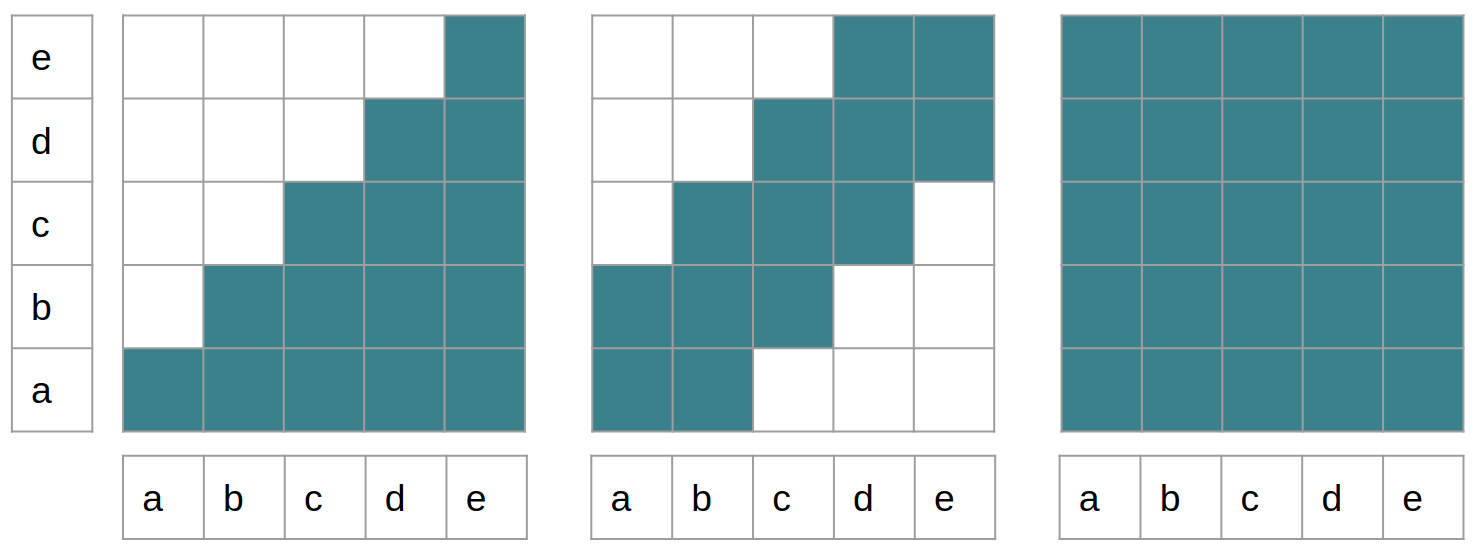
\includegraphics[width=\textwidth]{graphics/encoding.png}
\caption[Illustration of context range at each token in different encoding mechanism]{Illustration of context range at each token in different encoding mechanism. From left to right: Recurrent encoder, Convolution encoder, Attention-based encoder. The example sequence is $[a,b,c,d,e]$ and each colored column represent the context range of the corresponding token.}
\label{fig:attention}
\end{figure*}

The decoder takes the output of the encoder as one of it's inputs. The decoder works similarly to a language model as it predicts one token per time step. An Auto-regressive decoder conditions its prediction on the predictions of previous steps and the source sequence. Because all of our experiments use Auto-regressive NMT, from now a decoder is an auto-regressive decoder if there is not any other specification. The decoder has to take into account the hidden states of prediction history and the hidden state of source sentence to compute the current hidden state. The decoder also

NMT's Encoder/Decoder is usually a stack of multiple layers. As described above, the input source sequence is mapped to a sequence of word embeddings. This is considered as $0^{th}$ layer of the Encoder. The $i^{th}$ layer is built upon the $(i-1)^{th}$ layer by applying the same encoding mechanism (recurrent layer, convolution layer or self-attention layer) to the output of the $(i-1)^{th}$. However the parameters of different layers are not shared. The number of the stacked layers in of neural network model represent its depth while the width of a neural network is number of channels of each layer, i.e. the dimension of the hidden states in NMT's encoder/decoder. A neural network increases its capacity by increasing its width and depth.

\section{Recurrent NMT} \label{sec:rrn}
\nomenclature[rnn]{RNN}{Recurrent neural network}
This section reviews the very first NMT architecture, which is Recurrent Neural Network. The RNN encoder usually encodes the input sentence into a context vector of a fixed length. This representation is expected to be a good summary of the meaning of the whole source sequence. The RNN decoder will generate the prediction from the context vector. The variants in the RNN category are different only in functions used to map sentences to latent spaces.

\subsection{GRU, LSTM}
\nomenclature[gru]{GRU}{Gated Recurrent Unit}
\nomenclature[lstm]{LSTM}{Long-short term memory}
GRU and LSTM are the 2 most popular architectures in the group RNN. GRU stands for Gated Recurrent Unit while LSTM stands for Long Short Term Memory. Even though these architectures are in the same group, they are quite different in how they encode sentences. As we know, after mapping a source/target sentence to a sequence of word embeddings, the encoder/decoder uses GRU or LSTM to entangle the sequence of word embeddings producing highly abstract structures called contextualized embeddings. The encoding process goes from left to right, token by token. LSTM, which was first introduced by \cite{Hochreiter97long}, uses 4 gate
functions including input gate i, output gate o, forget gate f and memory cell c. At each time step t, the contextualized embedding $h_t$ is computed as follows.
\begin{equation}
\label{eq:lstm}
\begin{array}{rcl}
f_t &=& \sigma_g (W_f x_t + U_f h_{t-1} + b_f)\\
i_t &=& \sigma_g (W_i x_t + U_i h_{t-1} + b_i)\\
o_t &=& \sigma_g (W_o x_t + U_o h_{t-1} + b_o)\\
\tilde{c}_t &=& \sigma_c (W_o x_t + U_o h_{t-1} + b_o)\\
c_t &=& f_t \odot c_{t-1} + i_t \odot \tilde{c}_t\\
h_t &=& o_t \odot \sigma_h(c_t)\\
\end{array}
\end{equation}
where $x_t$ is word embedding of $t^{th}$ token, $\sigma_g$ is sigmoid function, $\sigma_c$ is hyperbolic tangent function, $\sigma_h$ is either hyperbolic tangent function or identity function and $\odot$ is element-wise multiplication. These functions are applied element-wise to intermediate vectors in the equations.

The motivation behind this highly complex structure is to stabilize the exploding/diminishing gradients propagating during back-propagation through the network or particularly back-propagation through time (BPTT \nomenclature[bptt]{BPTT}{Back-propagation through time}) in the RNN network \citep{Pascanu13onthe}. The second architecture GRU, which was first introduced by \cite{Cho14properties} in an MT paper, mitigates the complexity of LSTM by using only three gate functions as follows.
\begin{equation}
\label{eq:gru}
\begin{array}{rcl}
z_t &=& \sigma_g (W_z x_t + U_z h_{t-1} + b_z)\\
r_t &=& \sigma_g (W_r x_t + U_r h_{t-1} + b_r)\\
\hat{h}_t &=& \sigma_h (W_h x_t + U_h (r_t \odot h_{t-1})+b_h)\\
h_t &=& (1-z_t)\odot h_{t-1} + z_t \odot \hat{h}_t\\
\end{array}
\end{equation}

Where $\sigma_h$ is a hyperbolic tangent function while other notations are the same as in the equations of LSTM.

\subsection{Bidirectional encoder}
Unlike the decoder, the encoder is not obliged to process the input sequence from left to right. Effectively, the context of one token in the source sequence contains not only its preceding neighbors but also its following neighbors. Therefore, encoding the source sequence from left to right is not enough to cover the context of each token. To increase the coverage of contextualized embedding, the encoder process the source sequence both from left to right and from right to left at the same time, therefore becomes a bidirectional encoder. Bidirectional encoding results in two sequences of contextualized embeddings; the encoder simply combines two contextualized embeddings of a token into one real vector via either concatenation or summation. The resulting contextualized embedding captures information of every word in the source sequence around its corresponding token. 

\subsection{Attention mechanism \label{ssec:attention}}
Attention mechanism consists 3 components: Query vectors, Key vectors and Value vectors. Given a sequence $Q_i$, $i \in [1 \cdots n]$, $K_j$, $j \in [1 \cdots m]$ and $V_j$, $j \in [1 \cdots m]$, the results
of the attention mechanism composed by those vectors will be as follow.
\begin{equation}
Attention(Q,V,K)_i = \displaystyle{\mathop{\sum}_{j=1}^{m}} \frac{exp(sim(Q_i,K_j))}{\displaystyle{\mathop{\sum}_{p=1}^{m}}exp(sim(Q_i,K_p))}*V_j, i \in [1, \cdots, m]
\end{equation}
Where function $sim(x,y)$ can be a simple dot product $<x,y>$ \citep{Vaswani17attention}, a generalized dot product $<x,W_a*y>$ or $<v_a,tanh(W_a*[x,y])>$ \citep{Luong15stanford, Bahdanau15learning}.

The attention mechanism manages and quantifies the dependence between the input sequence and the output sequence (e.g., source contextualized embeddings and target contextualized embeddings), or the input sequence itself (e.g., self-attention layers in Transformer \citep{Vaswani17attention}). In the RNN MT model, the attention mechanism is used to capture the dependence of each token in the target sequence on the tokens in the source sequence. For example, \cite{Bahdanau15learning} computes a context vector at $i^{th}$ time step in the decoder as follows.
\begin{equation}
\begin{array}{rcl}
c_i &=& \sum_{j} \alpha_{ij} h_j \\
\alpha_{ij} &=& \frac{exp(e_{ij})}{\sum_{k}exp(e_{ik})} \\
e_{ik} &=& sim(s_{i-1},h_k)\\
\end{array}
\end{equation}
where $h_j$ is the output of the last layer of the encoder, $s_{i-1}$ is the hidden state at $(i-1)^{th}$ time step of the last layer of the  decoder. This context vector will be used to compute the hidden state at $i^{th}$ position by Attention mechanism improves the translation quality of very long sentences. Indeed, the context vector produced by the RNN encoder struggles to capture all the dependence between tokens  of the input sentence because it lacks the direct links between 2 tokens. The information of a token vanishes while the encoder moves toward the far ending of the input sequence. The same problem happens with the decoder when it decodes the context vector into the output sequence. The attention mechanism provides the direct links from each output token to any input token, allows the decoder to capture the information of any input token regardless of its position.

\section{Convolution NMT} \label{sec:cnn}
\nomenclature[cnn]{CNN}{Convolution neural network}
Convolution neural network was successfully applied to MT task in the work of \cite{Ghering17convolutional} that outperformed the current state-of-the-art performance of the RNN MT. In the CNN MT model, the CNN encoder and CNN decoder use convolution kernel to encode k consecutive tokens and iteratively move the convolution window from the beginning of the input sentence to the end of the sequence. We will not describe the details of the CNN MT because we did not use this architecture in the experiments of the thesis. However, we can briefly describe one layer in the CNN MT as follows.
\begin{equation}
\begin{array}{lcr}
h^l_i = v\bigg( W^l \big[h^{l-1}_{i-\frac{k}{2}}, \cdots, h^{l-1}_{i+\frac{k}{2}} \big] + b_w \bigg)
\end{array}
\end{equation}
where $h^l_i$ is the contextualized embedding of $i^{th}$ token in the $l^{th}$ layer, the function v is Gated Linear Unit \citep{Ghering17convolutional}. In the decoder, CNN MT also uses attention mechanism to improve the performance on the long sentences. 

To prevent the future information in the prediction of a token, one
pads $k-1$ in the left side of the output sequence, e.g $PAD$, $PAD$,$ <BOS>$,$je$,$t'$,$aime$ for convolution kernel of size 3 so that $\big[ PAD, PAD, <BOS>\big]$ predicts $je$, $\big[ PAD,<BOS>,je\big]$ predicts $t'$ etc.

\section{Attention-based NMT} \label{sec:transformer}
Transformer architecture was first introduced by \cite{Vaswani17attention} and has quickly become the state-of-the-art architecture not only in MT but also in language modeling (LM)\cite{Devlin19bert,Brown20language,Conneau19cross}, text summarization \cite{Zhang20pegasus} etc. The Transformer model's power relies on the attention mechanism, which was discussed in the previous section \ref{ssec:attention}. The Transformer model consists of a fully attention-based encoder and decoder. 
\subsection{Transformer encoder}
The Transformer encoder consists of layers made of a multi-head self-attention sub-layer followed by a position-wise fully connected feed-forward network. The multi-head self-attention sub-layer is an extension of the self-attention sub-layer and is described by the following equation.
\begin{equation}
\begin{array}{rcl}
MultiheadAttention\big( Q,V,K \big) &=& Concat \big[ head_0, \cdots , head_h \big] W_0\\
head_i &=& Attention \big( QW_i^Q, VW_i^V, KW_i^K \big)\\
\end{array}
\end{equation}

Where $W_i^Q, W_i^V, W_i^K \in \mathbb{R}^{d_k \times d_h}$ with $d_h \times h = d_k$, $d_k$ is the dimension of word embedding space and also the size of Transformer model. Unlike the version in the section \ref{ssec:attention}, the attention mechanism is simply as follows.
\begin{equation}
Attention\big( Q, V, K \big) = Softmax\big(\frac{Q K^T}{\sqrt{d_k}} \big) V
\end{equation}
The feed-forward network is designed as follows.
\begin{equation}
FFN(x) = ReLu(xW_1+b_1)W_2+b_2
\end{equation}
Where $W_1 \in \mathbb{R}^{d_k \times d_b}$,$W_2 \in \mathbb{R}^{d_b \times d_k}$,$b_1 \in \mathbb{R}^{d_b}$,$b_2 \in \mathbb{R}^{d_k}$.
The final detail is that the output of each sub-layer has to pass through a Layer-Normalization sub-layer \citep{Jimmy16layer}. In conclusion, the contextualized embedding of the $l^{th}$ layer of the Transformer encoder will be as follows.
\begin{equation}
\begin{array}{rcl}
\tilde{h}^l &=& LN\bigg(Multihead\big(h^{l-1}, h^{l-1}, h^{l-1}\big) + h^{l-1}\bigg) \\ 
h^l &=& LN\bigg(FFN\big(\tilde{h}\big) + \tilde{h}\bigg)
\end{array}
\end{equation}

Where $LN$ is a Layer-Normalization sub-layer.
\subsection{Transformer decoder}
The Transformer decoder consists of layers made of a multi-head self-attention sub-layer followed by a multi-head cross-attention sub-layer then by a position-wise fully connected feed-forward network. The multi-head self-attention sub-layer and the feed-forward network have the same design as those in the Transformer encoder. The multi-head cross-attention sub-layer of the $l^{th}$ layer of the decoder uses the output of the last layer of the encoder as keys and values, the output of the $l^th$ self-attention sub-layer as queries.
\begin{equation}
\begin{array}{rcl}
\tilde{s}^l &=& LN\bigg( Multihead\big( s^{l-1},s^{l-1},s^{l-1} \big) + s^{l-1} \bigg) \\
\bar{s}^l &=& LN\bigg( Multihead\big( \tilde{s}^l, h^u, h^u \big) + \tilde{s}^l \bigg) \\
s^l &=& LN\bigg( FFN\big( \bar{s}^l \big) + \bar{s}^l \bigg) \\
\end{array}
\end{equation}
where $s^l$,$s^{l-1}$ are the outputs of the $l^{th}$ and $(l-1)^{th}$ layers of the decoder respectively, $h^u$ is the output of the last layer of the encoder.

In order to prevent the future information in the decoder, at each time step $i^{th}$, the attention scores of tokens at positions after $i^{th}$ are masked by zero.

\subsection{Positional embedding}
Transformer encoder and decoder both do not their corresponding input sequence in one direction but fully connects all pair of tokens in the same time, therefore the order of the sequence is not taken into account. In order to represent the position of tokens in the sequence, \cite{Vaswani17attention} proposed the use of positional embedding. Given the size of word embedding $d_k$ , the positional embedding of position $i^{th}$ is defined as follows
\begin{equation}
\begin{array}{rcl}
PE\big(pos,2i\big) &=& sin \big( \frac{pos}{1000^{\frac{2i}{d_k}}} \big)\\
PE\big(pos,2i+1\big) &=& cos \big( \frac{pos}{1000^{\frac{2i}{d_k}}} \big)\\
\end{array}
\end{equation}

The positional embedding will be added to the corresponding word embedding of the $i^{th}$ token of the input sequence.
\section{NMT training} \label{sec:train}
The values of the parameters in the NMT model is estimated by gradient descent method \citep{Nesterov14introductory}, which is one of the oldest approaches in the Optimization area \citep{Cauchy1847method}. The loss function is the traditional cross-entropy of the training data. 
\begin{equation}
L(\theta) = -\displaystyle{\mathop{\sum}_{x,y}}log P(y|x;\theta)
\end{equation}
The gradient is computed by back-propagation algorithm \citep{Rumelhart88learning}. Like many deep learning models, the NMT model is usually trained with a massive amount of data that makes the gradient descent method is not computationally plausible. Therefore, stochastic gradient descent is proposed to mitigate the computational burden of large-scale models \citep{Herbert51stochastic,Kiefer52stochastic,Bottou10large}. However, Deep Neural networks are usually much harder to train because of their size and their complex structure \cite{Pascanu13onthe,Glorot10understanding}. Many approaches are proposed to facilitate the training of deep models such as Gradient clipping \citep{Pascanu13onthe}, Truncate back-propagation \citep{Jaeger02tutorial}, Normalization methods \citep{Ioffe15batch,Jimmy16layer}, Residual connections \citep{He16deep}, Noam schedule \citep{Vaswani17attention} etc.

\section{Decoding algorithm} \label{sec:inference}
The NMT model basically models the conditional probability $P(y|x)$of the translation sentence $y$ given the input sentence $x$. The prediction of the NMT model is the sentence with the highest conditional probability.

\begin{equation}
\hat{y} = \displaystyle{\mathop{\argmax}} P(y|x;\theta)
\end{equation}

However, the search space of $y$ is infinitely large, causing the implausibility of the exact search. Beam search \citep{Och98improving} is the most common decoding algorithm in Neural Machine Translation and Statistical Machine Translation. 

Beam search starts with K empty hypotheses, which are initialized by "begin of sentence" token $<BOS>$. For the $i^{th}$ current hypothesis $[y^{i}_{<t}]$, the top-K tokens, with the highest conditional probabilities $P(y_t = a_i | y_{<t},x;\theta)$, are picked and appended to the current hypothesis. The search space, therefore, is extended to $K*K$ hypotheses. Beam search selects only the top $K$ hypotheses from these $K*K$ hypotheses. Beam search stops extending the completed hypotheses, which are ended with the "end of sentence" token $<EOS>$ or reach the predefined length limit. Beside the left-to-right decoding, there are several variant decoding direction including non-monotonic decoding \citep{Welleck19non}, non auto-regressive decoding \citep{Jiatao17non}, synchronous bidirectional decoding \cite{Zhou19synchronous}. Because the decoding algorithms are not included in this research topic, we would like to be limited to this brief description.
\nomenclature[eos]{EOS}{end-of-sentence}

\section{MT evaluation}







































